\chapter{Extra Information} \label{chap:a}

This appendix contains tables, various images of files, and maps to better illustrate the topics discussed throughout the report.
\vspace{15pt}
\begin{table} [h] \label{tab1}
    \centering
    \begin{tabular}{||c c c c||} 
         \hline
 \textbf{Attribute} & \textbf{Min Value} & \textbf{Max Value} & \textbf{Rounding Value} \\ [0.5ex] 
 \hline\hline
cloudiness & 0 & 100 & 3 \\
\hline
precipitation & 0 & 100 & 3 \\
\hline
precipitation deposits & 0 & 100 & 3 \\
\hline
wind intensity & 0 & 100 & 3 \\
\hline
sun azimuth angle & 0 & 360 & 3 \\
\hline
sun altitude angle & -90 & 90 & 3 \\
\hline
fog density & 0 & 100 & 3 \\
\hline
fog distance & 0 & +$\infty$ & 3 \\
\hline
wetness & 0 & 100 & 3 \\
\hline
fog falloff & 0 & +$\infty$ & 3 \\
\hline
scattering intensity & 0 & +$\infty$ & 3 \\
\hline
mie scattering scale & 0 & +$\infty$ & 3 \\
\hline
rayleigh scattering scale & 0 & +$\infty$ & 3 \\
\hline
dust storm & 0 & 100 & 3 \\
 \hline
    \end{tabular}
    \caption{Weather related scenario attributes}
    \label{tab:weather_attributes}
\end{table}

\begin{table} \label{tab2}
    \centering
    \begin{tabular}{||c c c c||} 
    \hline
 \textbf{Attribute} & \textbf{Min Value} & \textbf{Max Value} & \textbf{Rounding Value} \\ [0.5ex] 
\hline\hline
number of pedestrians & 0 & +$\infty$ & 0 \\
\hline
number of vehicles & 0 & +$\infty$ & 0 \\
\hline
number of two wheel vehicles & 0 & +$\infty$ & 0 \\
\hline
proportion of speeding vehicles & 0 & 1 & 3 \\
\hline
proportion of vehicles without lights & 0 & 1 & 3 \\
\hline
proportion of light ignoring vehicles & 0 & 1 & 3 \\
\hline
light ignoring percent & 0 & 100 & 3 \\
\hline
proportion of sign ignoring vehicles & 0 & 1 & 3 \\
\hline
sign ignoring percent & 0 & 100 & 3 \\
\hline
proportion of vehicle ignoring vehicles & 0 & 1 & 3 \\
\hline
vehicle ignoring percent & 0 & 100 & 3 \\
\hline
proportion of walker ignoring vehicles & 0 & 1 & 3 \\
\hline
walker ignoring percent & 0 & 100 & 3 \\
\hline
proportion of keeping right vehicles & 0 & 1 & 3 \\
\hline
keeping right percent & 0 & 100 & 3 \\
\hline
proportion of lane changing vehicles & 0 & 1 & 3 \\
\hline
lane change percent & 0 & 100 & 3 \\
\hline
proportion of misbehaving pedestrians & 0 & 1 & 3 \\
\hline
proportion of running pedestrians & 0 & 1 & 3 \\
\hline
proportion of road crossing pedestrians & 0 & 1 & 3 \\
\hline
number of junctions & 0 & +$\infty$ & 0 \\
\hline
distance in metres & 0 & +$\infty$ & 3 \\
\hline
area in square metres & 0 & +$\infty$ & 3 \\ [1ex] 
\hline
difficulty & 0 & 1000 & 3 \\ [1ex] 
\hline
    \end{tabular}
    \caption{Traffic related scenario attributes}
    \label{tab:traffic_attributes}
\end{table}


\begin{figure}
    \centering
    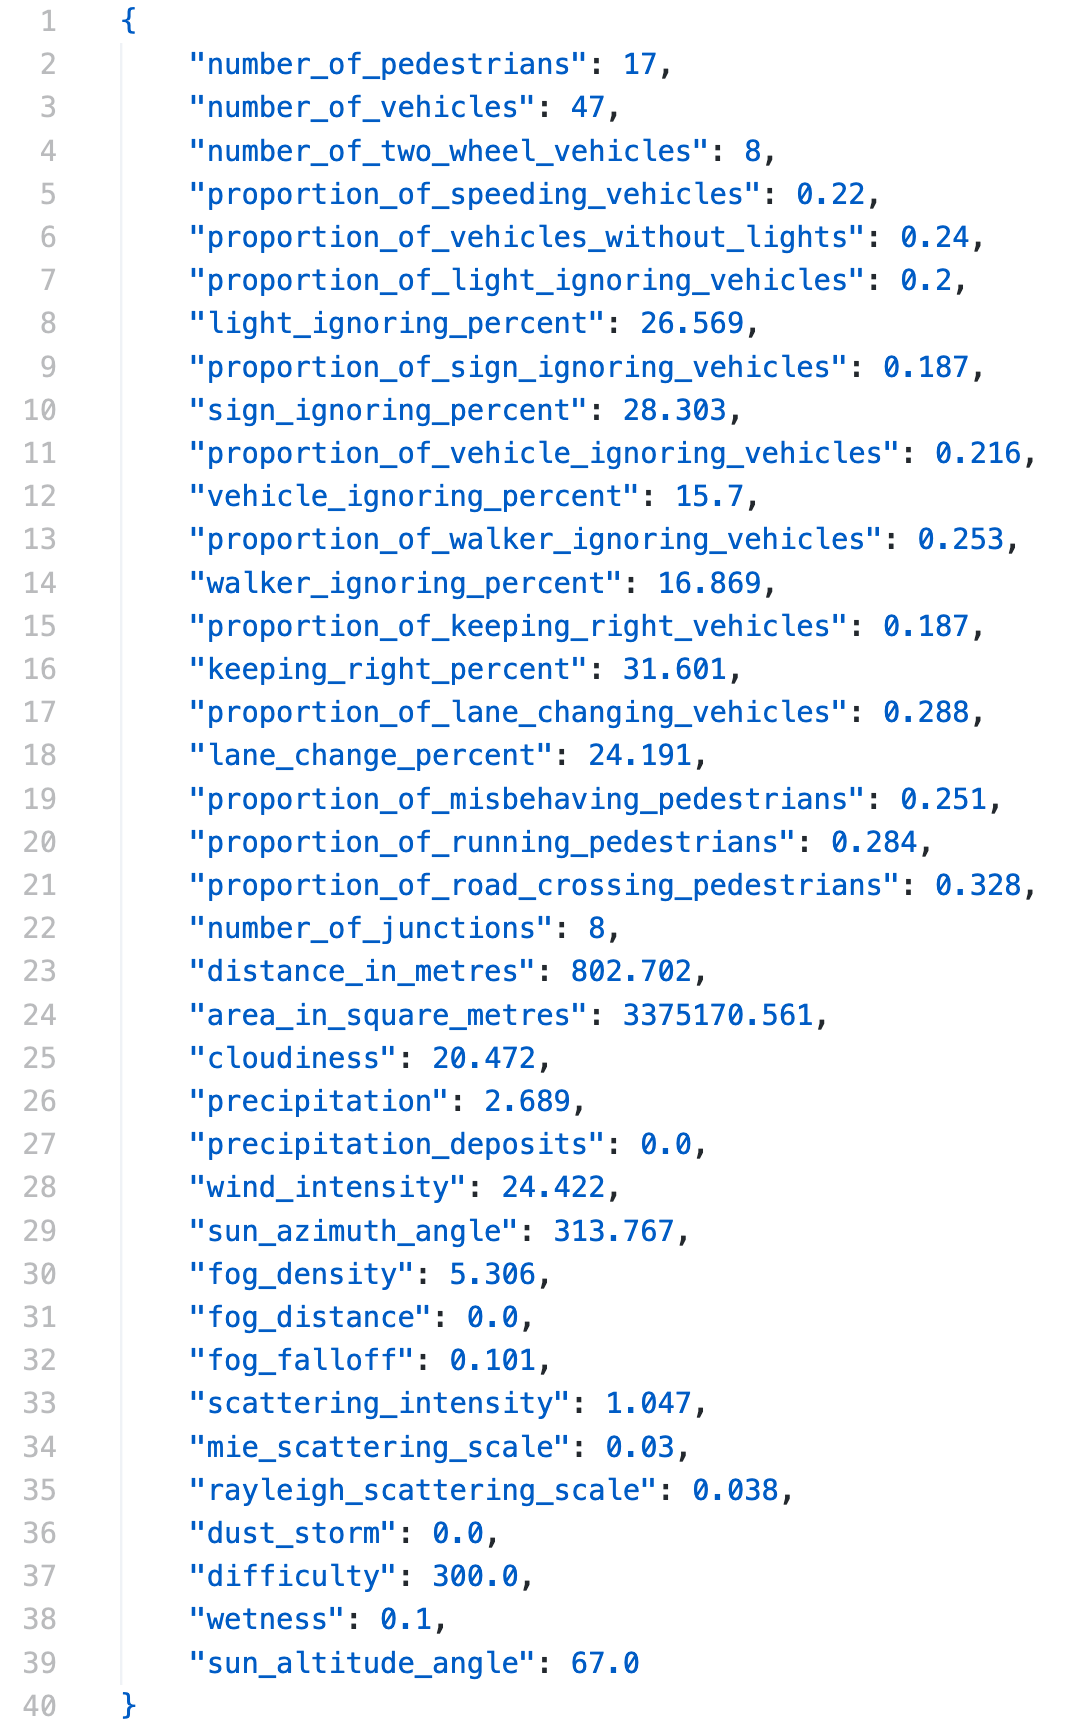
\includegraphics[width = 0.7\textwidth]{research_paper/Images/generated_scenario.png}
    \caption{Example of a generated scenario}
    \label{fig:generated_scenario}
\end{figure}

\begin{figure}
    \centering
    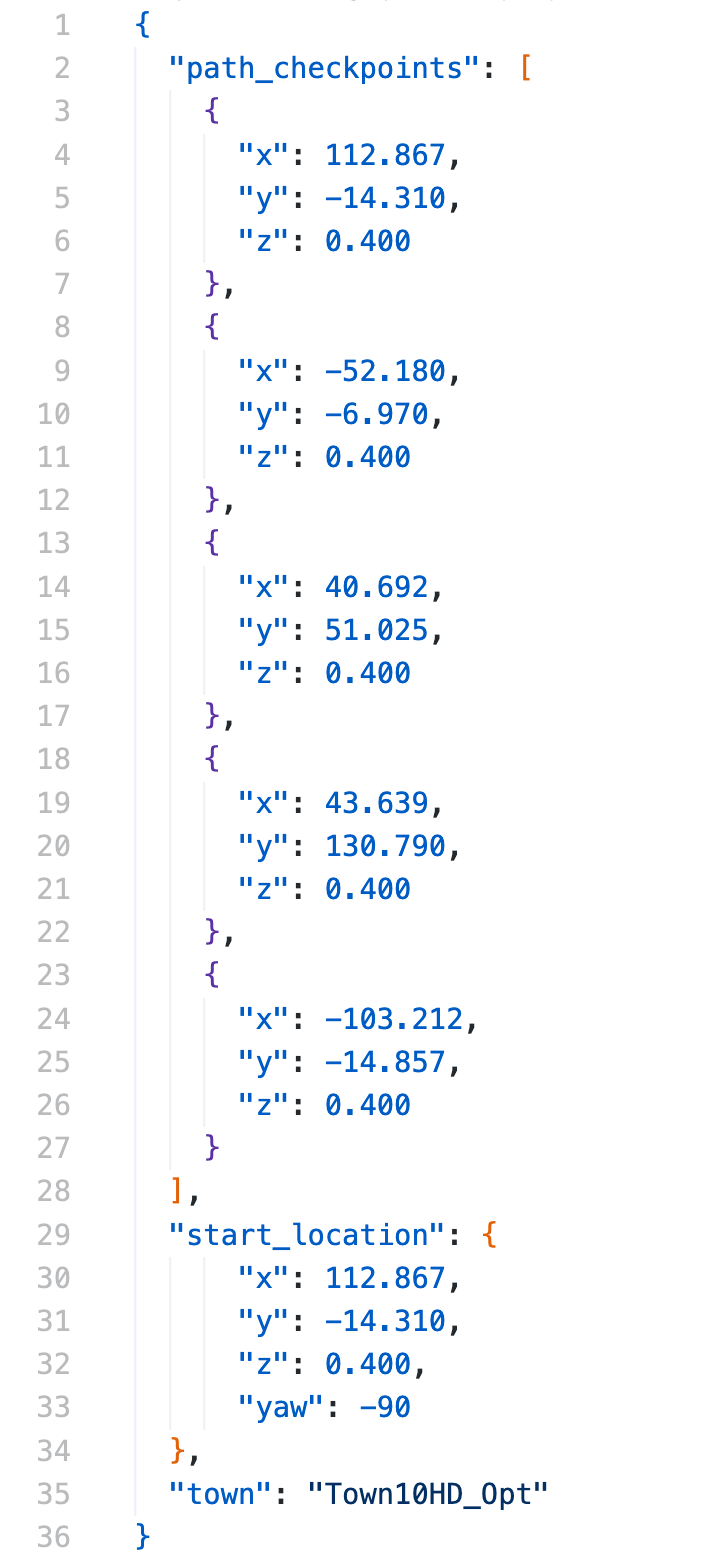
\includegraphics[width = 0.5\textwidth]{research_paper/Images/generated_path.png}
    \caption{Example of a generated path}
    \label{fig:generated_path}
\end{figure}

\begin{figure}
    \centering
    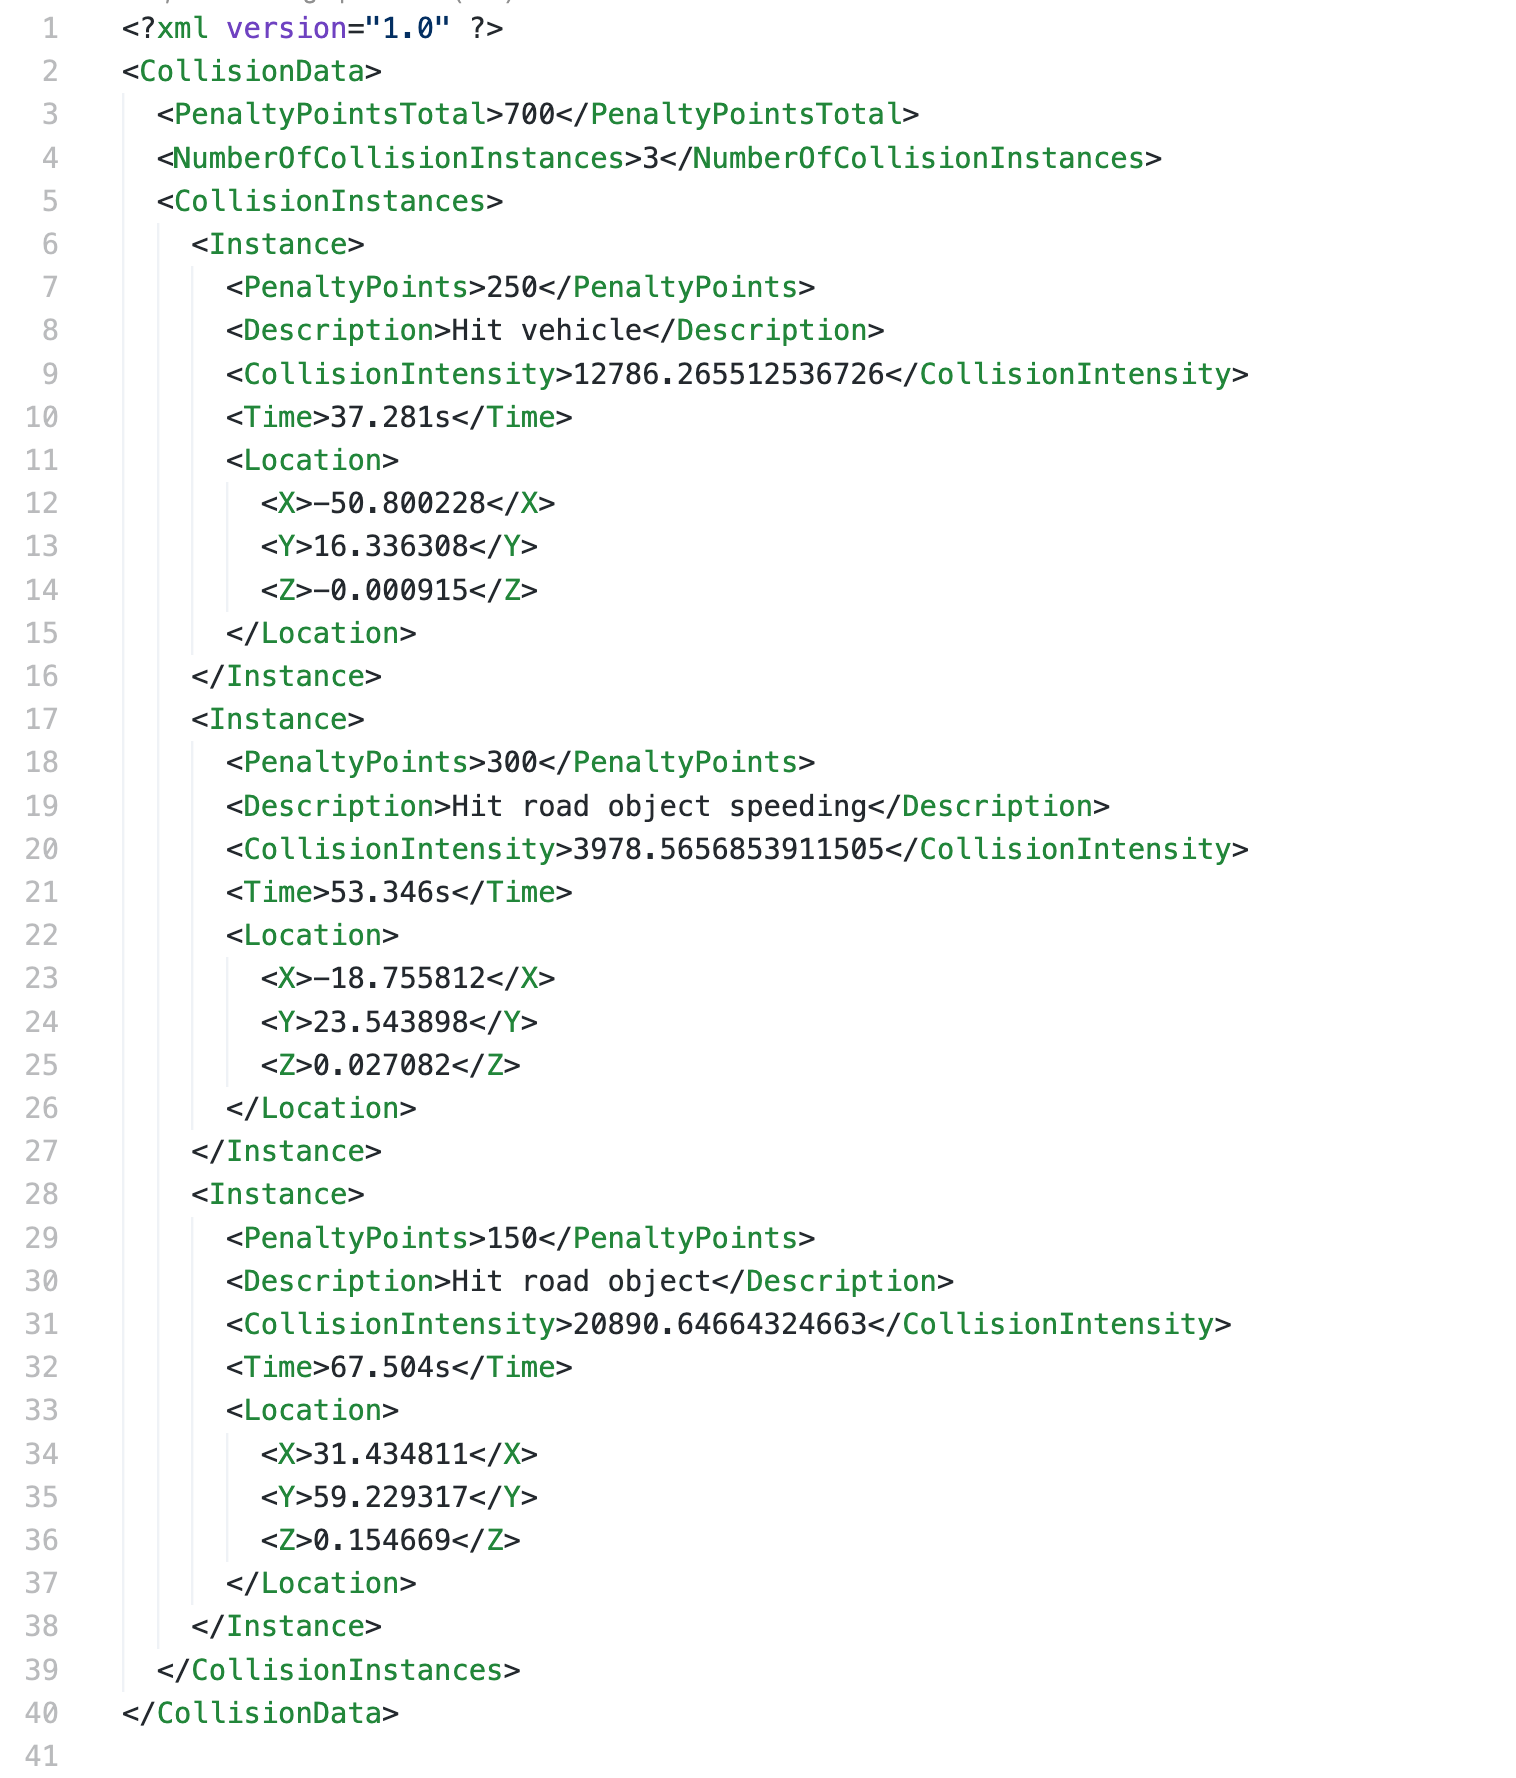
\includegraphics[width = 0.86\textwidth]{research_paper/Images/collision_data.png}
    \caption{An example of collision\_data.xml file structure}
    \label{fig:collision_data}
\end{figure}

\begin{table}
    \centering
    \begin{tabular}{||c c c||} 
         \hline
 \textbf{Category} & \textbf{Not speeding} & \textbf{Speeding} \\ [0.5ex] 
 \hline\hline
No beams and no fog lights & 50 & 50 \\
No beams & 30 & 30 \\
No fog lights & 10 & 10 \\
Hit pedestrian & 600 & 1200 \\
Hit vehicle & 250 & 500 \\
Hit two-wheel vehicle & 400 & 800 \\
Hit road object & 150 & 300 \\
Red light violation & 50 & 100 \\
Stop sign/marking violation & 40 & 80 \\
Solid lane marking & 20 & 60 \\
Double solid lane marking & 40 & 100 \\
Broken lane marking no turn indicator & 10 & 30 \\
Light speeding & 1 & 1 \\
Heavy speeding & 3s & 3 \\
 \hline
    \end{tabular}
    \caption{Penalty score table}
    \label{tab:penalty_values}
\end{table}

\begin{figure}
    \centering
    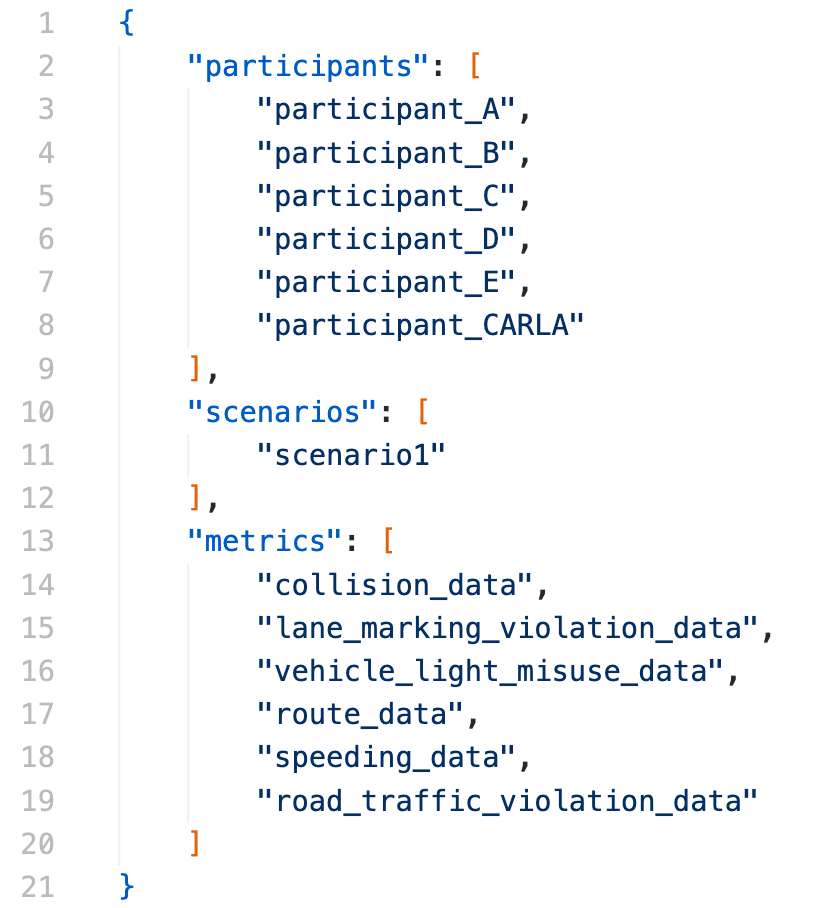
\includegraphics[width = 0.7\textwidth]{research_paper/Images/analysis_parameters.png}
    \caption{An example of analysis\_parameters.json file}
    \label{fig:analysis_parameters}
\end{figure}

\begin{figure}
    \centering
    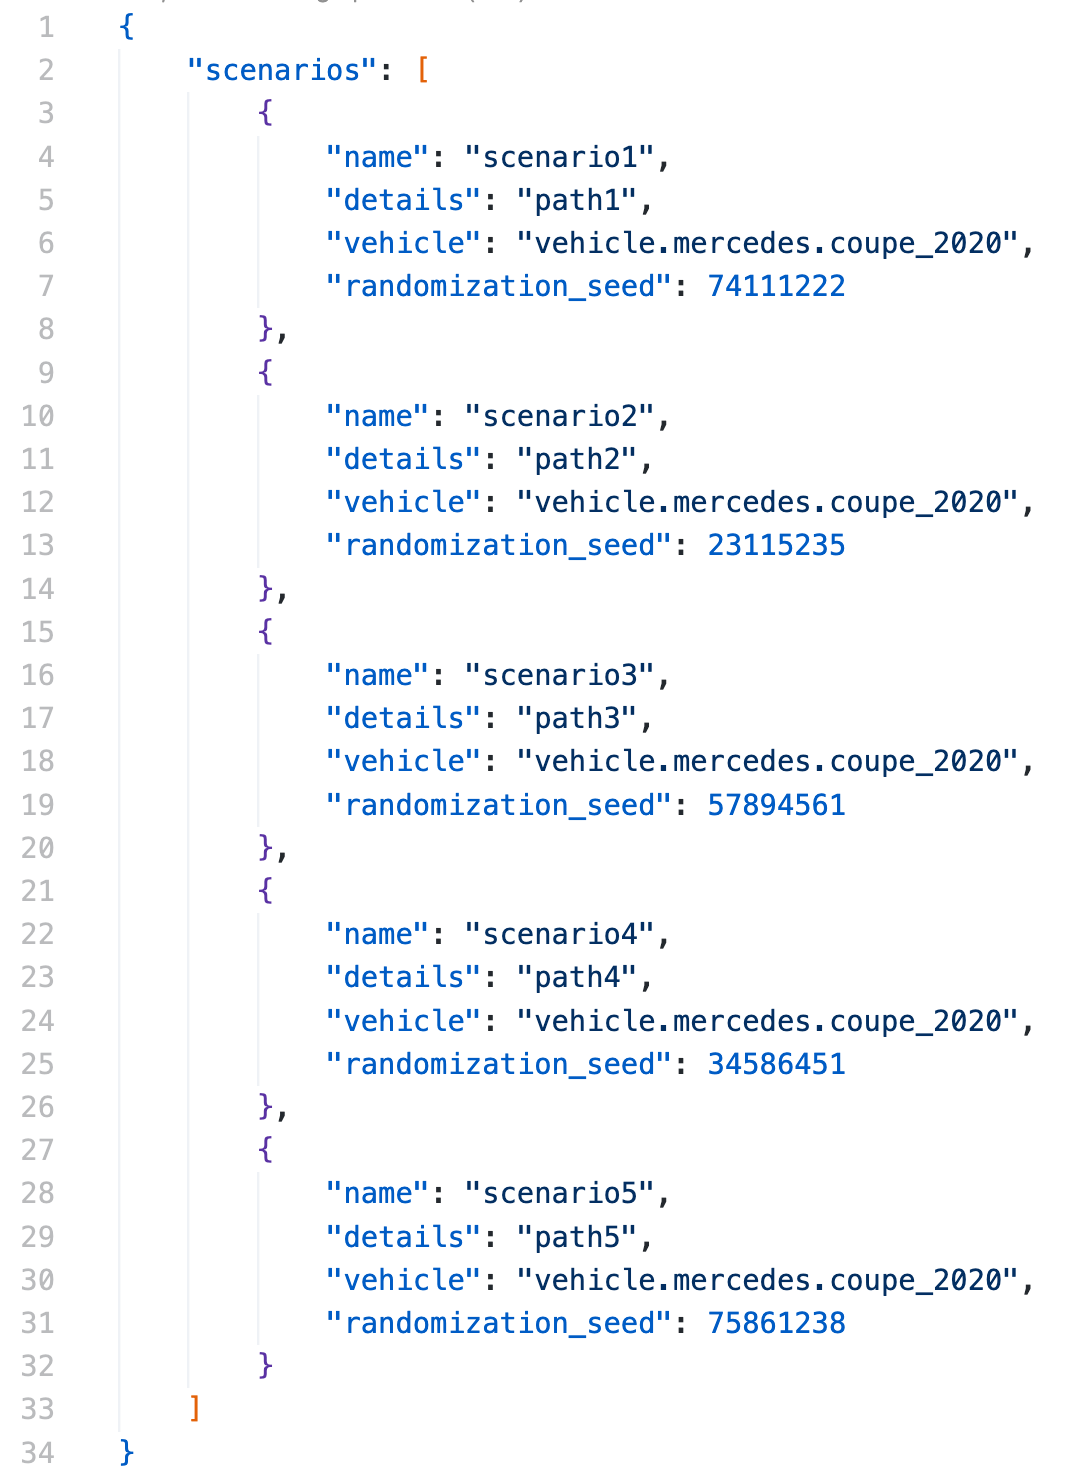
\includegraphics[width = 0.8\textwidth]{research_paper/Images/scenario_list.png}
    \caption{An example of the scenario list}
    \label{fig:scenario_list}
\end{figure}

\begin{figure} [h]
    \centering
    \textbf{OS}: Ubuntu 20.04.4 LTS
    
    \textbf{CPU}: 11th Gen Intel Core i7-11700KF @ 3.60GHz $\times$ 16
    
    \textbf{RAM}: 64GB
    
    \textbf{GPU}: NVIDIA GeForce RTX 3090
    \caption{Technical specifications of the lab computer}
    \label{specs}
\end{figure}

\begin{figure}
    \centering
    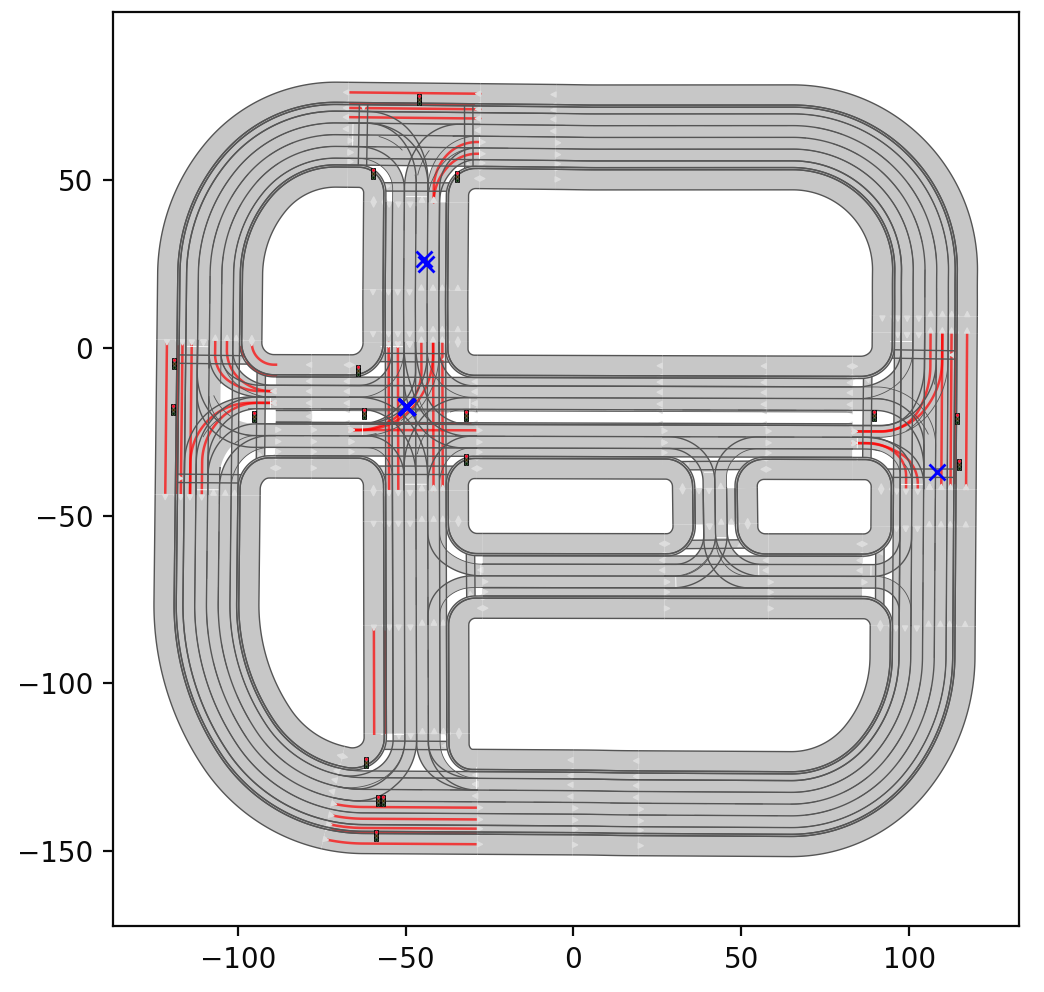
\includegraphics[width = 0.9\textwidth]{research_paper/Images/correctly_marked.png}
    \caption{Correctly marked collision locations}
    \label{fig:correctly_marked}
\end{figure}

\begin{figure}
    \centering
    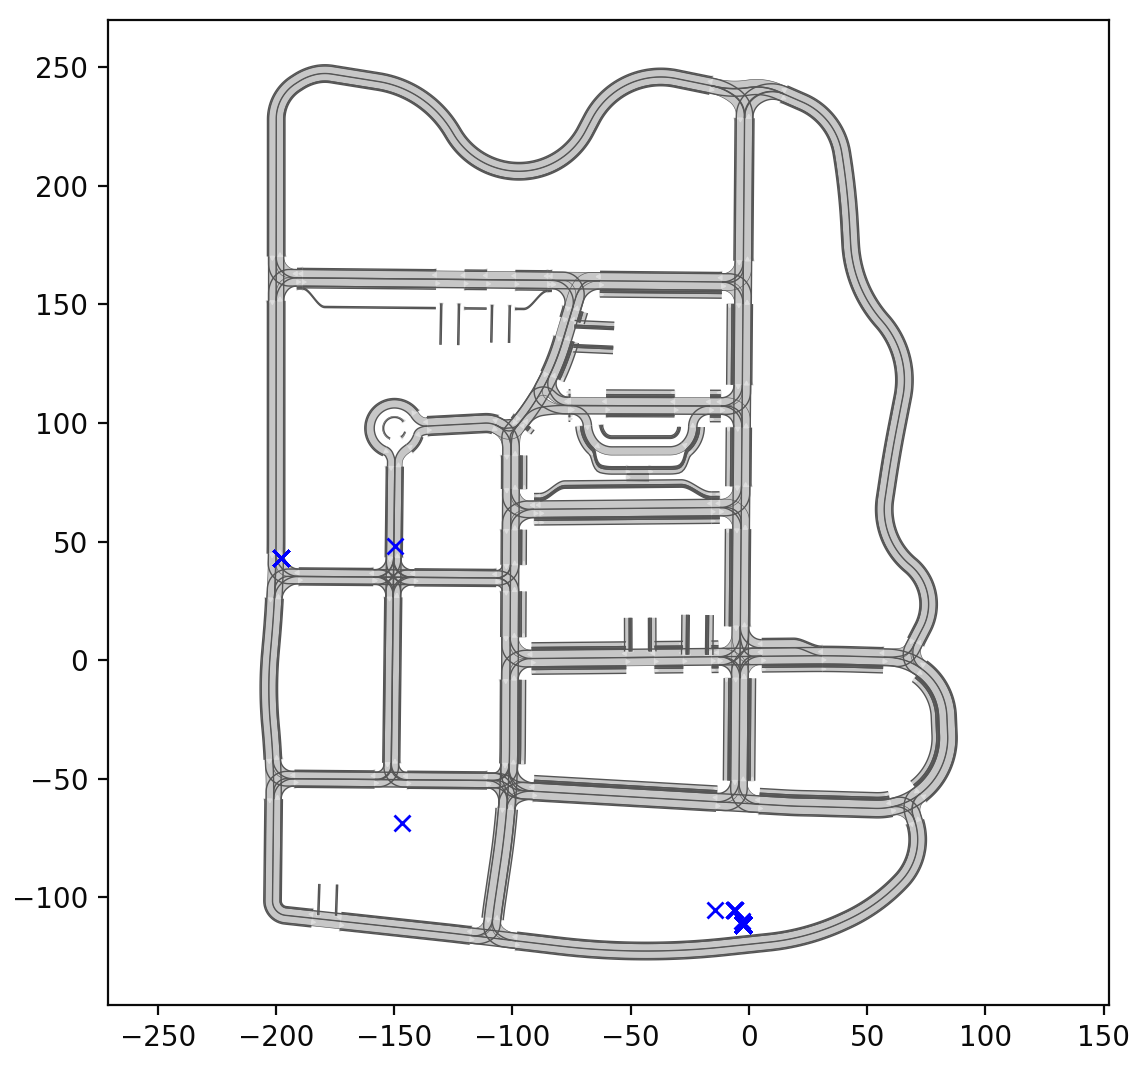
\includegraphics[width = 0.9\textwidth]{research_paper/Images/incorrectly_marked.png}
    \caption{Incorrectly marked collision locations}
    \label{fig:incorrectly_marked}
\end{figure}